\textit{Objet ? Objet-relationnel ou relationnel pur ? C'est dans cette phase de conception que nous allons répondre à cette question. Ensuite, une seconde partie décrira l'utilité des ORM, puis les templates de l'application seront présentés.}

\section{Une histoire de paradigmes}
\subsection{Le paradigme objet}

Le modèle objet pour le stockage des données présente les mêmes avantages que pour la programmation orienté objet, à savoir une grande capacité d'abstraction, de factorisation et de maintenance. Malheureusement ce modèle est implémenté par peu de SGBD (O2, db4o, ObjectStore) ce qui nuit grandement à la portabilité des applications basées sur celui-ci.

\subsubsection{Schéma objet}
\lstinputlisting[language=SQL,morekeywords={Class, extent, relationship, key, attribute, inverse}]{./sources/schema_objet.odl}

\subsection{Le paradigme objet-relationnel}

De nombreux SGBD tels que ORACLE offrent une vision hybride entre l'objet et le relationnel : l'objet-relationnel.

Ce modèle est standardisé par la norme SQL3. Cependant il n'est jamais implémenté dans sa globalité ce qui pose à nouveau un problème de portabilité : un script SQL pour ORACLE ne s'exécutera pas sur PostgreSQL.

\subsubsection{Schéma objet-relationnel}

Voici le script ORACLE de création des types et tables pour notre application, utilisant des aspects objet-relationnel.
\lstinputlisting[language=sql]{./sources/schema_objet_relationnel.sql}

\subsection{Le paradigme relationnel pur}

La vision historique des bases de données est le relationnel pur. Il offre des performances reconnus. En revanche, son utilisation peut poser problème lorsque la modélisation de l'application est faite en objet. Il faut alors créer un schéma relationnel à partir de la modélisation objet (Diagramme UML de classes), et développer des procédures de stockage afin de gérer la persistance des objets.

\subsubsection{Schéma relationnel}

Le schéma relationnel pur présenté ci-dessous permet la persistance des objets nécessaires à notre application. D'après le diagramme UML de classes, nous avons ajouté une table des synonymes et une table d'associations.

\begin{description}
\item[TERME](\underline{lib\_terme})
\item[CONCEPT](\underline{terme\_vedette}\up{\#}, concept\_general\up{\#})
\item[SYNONYME](\underline{terme\up{\#}, concept\up{\#}})
\item[ASSOCIATION](\underline{concept1\up{\#}, concept2\up{\#}})
\end{description}

\section{ORM}

	\subsection{Qu'est qu'un ORM?}
    Un ORM ou \emph{mapping objet-relationnel} (en anglais \emph{object-relational mapping}) est une méthode de programmation qui consiste à donner l'illusion d'une base de données orientée objet à partir d'une base de données relationnelle en implémentant une interface entre celle-ci et le code de l'application.
   
	\subsection{Pourquoi?}
    Nous avons vu que les systèmes de gestion de bases de données orientées objet sont actuellement peu nombreux, que la norme SQL3 n'est que partiellement implémentée, notamment sur le SGBD Postgresql que nous avons décidé d'utiliser.
    
En revanche, cette méthode d'abstraction présente l'inconvénient de générer un schéma différent de la vision objet avec laquelle est modélisée l'application. Il peut parfois être nécessaire d'intervenir directement sur la base de données (développement de TRIGGERS, dump SQL, \ldots), ce qui nécessite alors un effort d'analyse et de compréhension.

\section{Décisions}

\subsection{Postgresql}

Dès le lancement du projet, nous avons choisi de travailler avec Postpresql pour plusieurs raisons :
\begin{itemize}
\item découvrir l'objet-relationnel sur un nouveau système (autre qu'ORACLE, vu en TD/TP),
\item travailler avec un logiciel libre,
\item respectueux des standards SQL,
\item et précurseur aux débuts de l'objet-relationnel (premier SGBD à intégrer des aspects objet).
\end{itemize}

\subsection{Framework \& ORM}

Après discussion, nous avons choisi de travailler à l'aide du framework Symfony (version 2), intégrant l'ORM Doctrine (version 2). Ces outils seront présentés dans la partie suivante.

Les raisons qui nous ont poussé à faire le choix de développer l'application à l'aide d'un ORM sont les suivantes :
\begin{itemize}
\item nous avons pris conscience que l'application à développer ne nécessitait pas d'aspects objet (objet-relationnel),
\item nous tenions à travailler dans un environnement libre en utilisant Postgresql, mais aujourd'hui il ne fournit pas autant de fonctions orientées objet que ORACLE,
\item nous souhaitions travailler avec des technologies matures,
\item nous souhaitions découvrir la mise en place d'une application à l'aide d'un ORM.
\end{itemize}
	
	
\section{Templates et formulaires}

\subsection{Accueil}

La page d'accueil de l'application \emph{Thésaurus Rex} est composée d'un court texte de bienvenue. La partie gauche est composée du logo, d'un champs de recherche, et de deux liens d'accès aux parties de l'application : gestion des concepts et gestion des termes. Ce panel est visible sur toutes les vues.
\begin{figure}[H]
\begin{center}
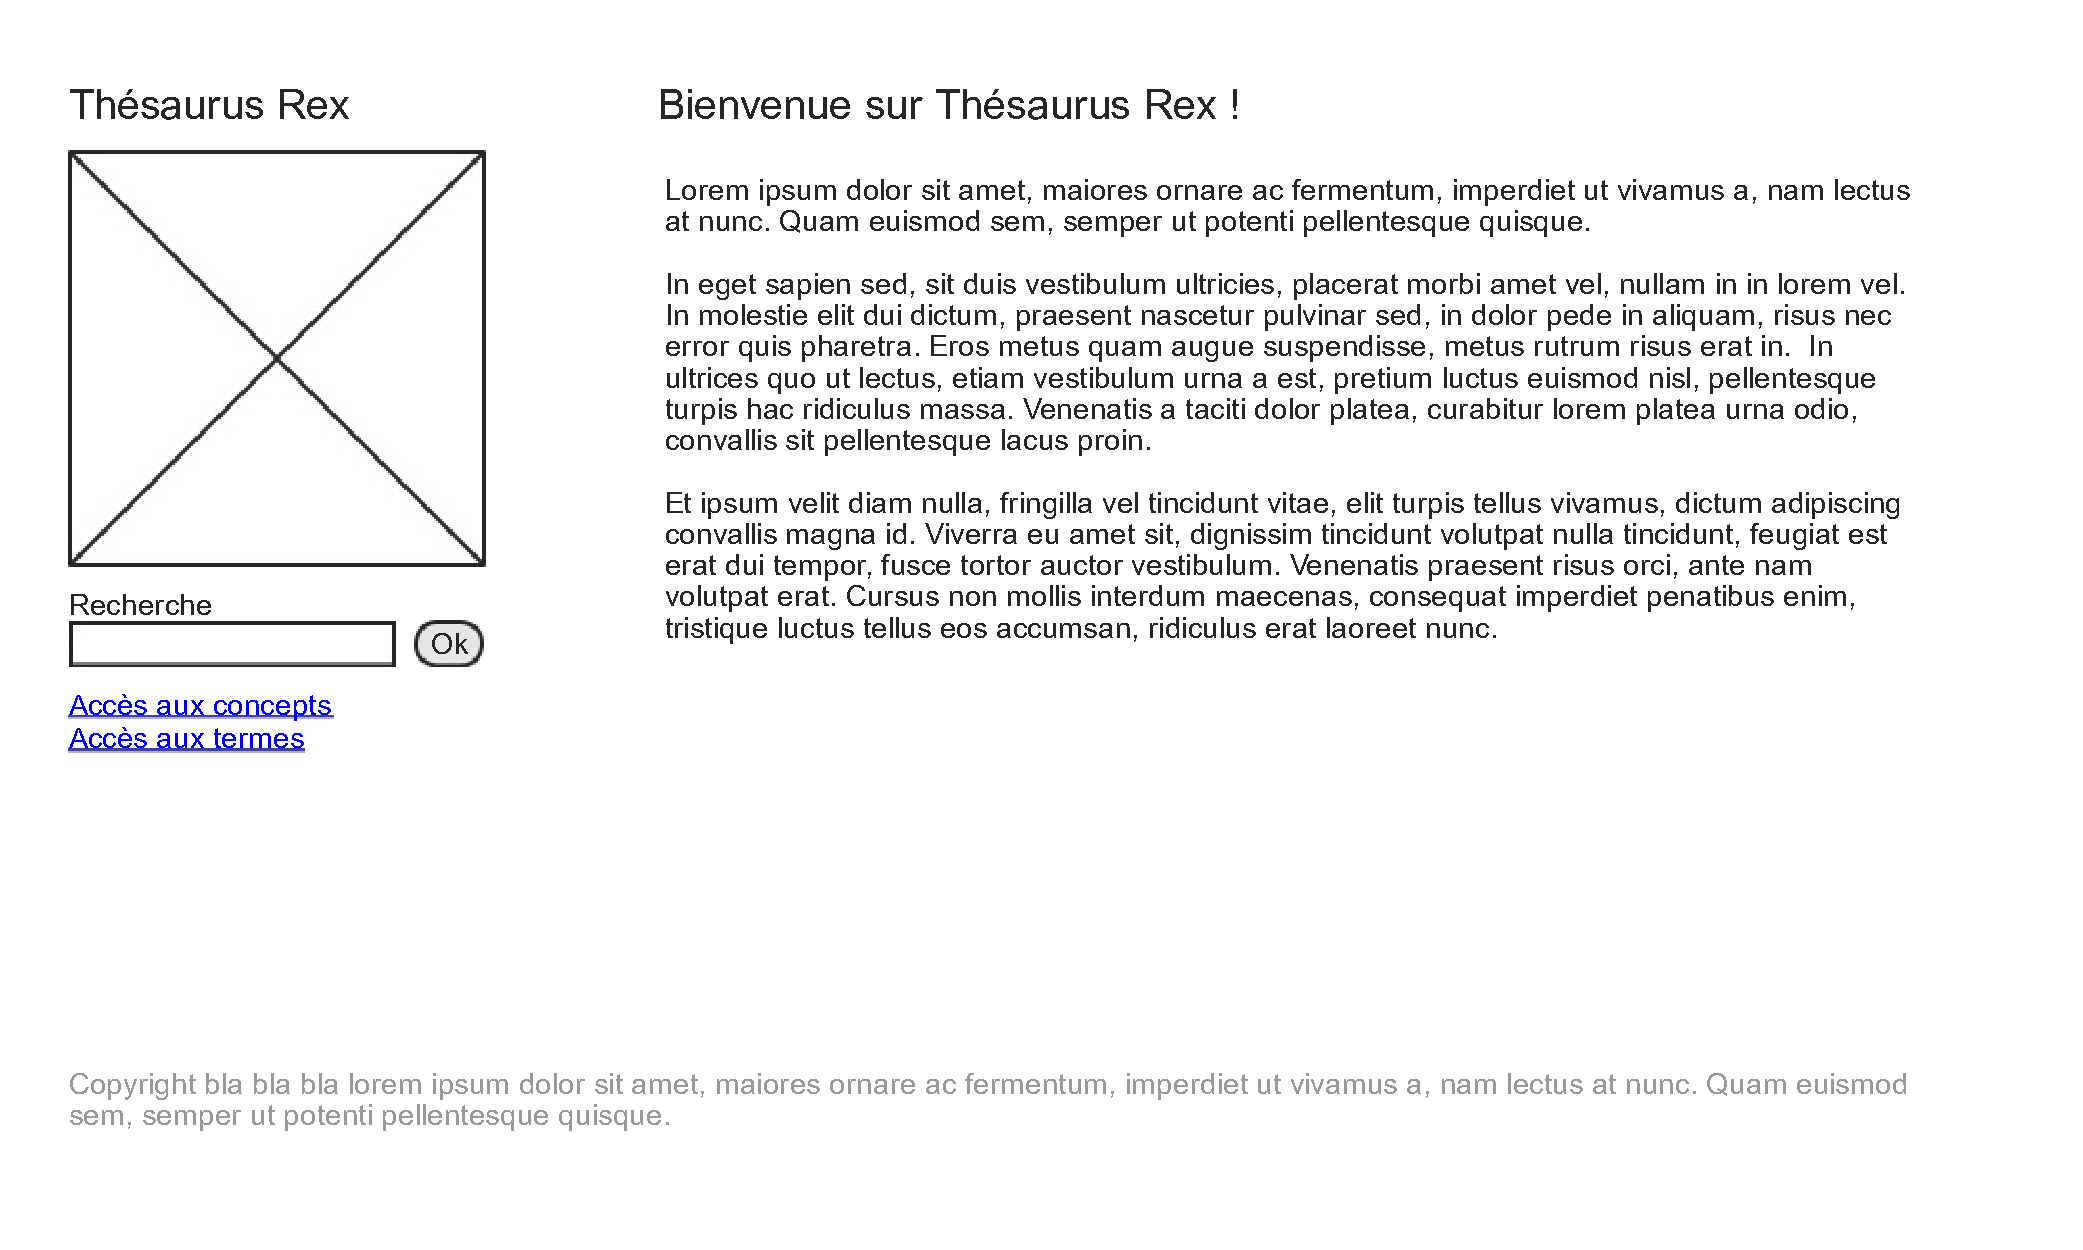
\includegraphics[width=\textwidth]{files/template_accueil}
\end{center}
\caption{Template de la page d'accueil de Thésaurus Rex.}
\end{figure}

\subsection{Vue hiérarchique des concepts}

La vue hiérarchique permet de visualiser l'ensemble des concepts sous la forme d'arbre en affichant le terme vedette de chaque concept. \emph{TG} signifie \emph{Terme Général},  il s'agit des racines de la hiérarchie (ils ne possèdent pas de concept général). \emph{TS} signifie \emph{Terme spécifique}, il s'agit des concepts possédant un terme général.

Notons que nous avons utilisé \emph{Termes Général} et \emph{Termes Spécifique} au lieu du mot \emph{Concept}. En effet, bien que ces deux notions sont différentes, dans le cas de la vue hiérarchique, il est envisageable des les confondre.
\begin{figure}[H]
\begin{center}
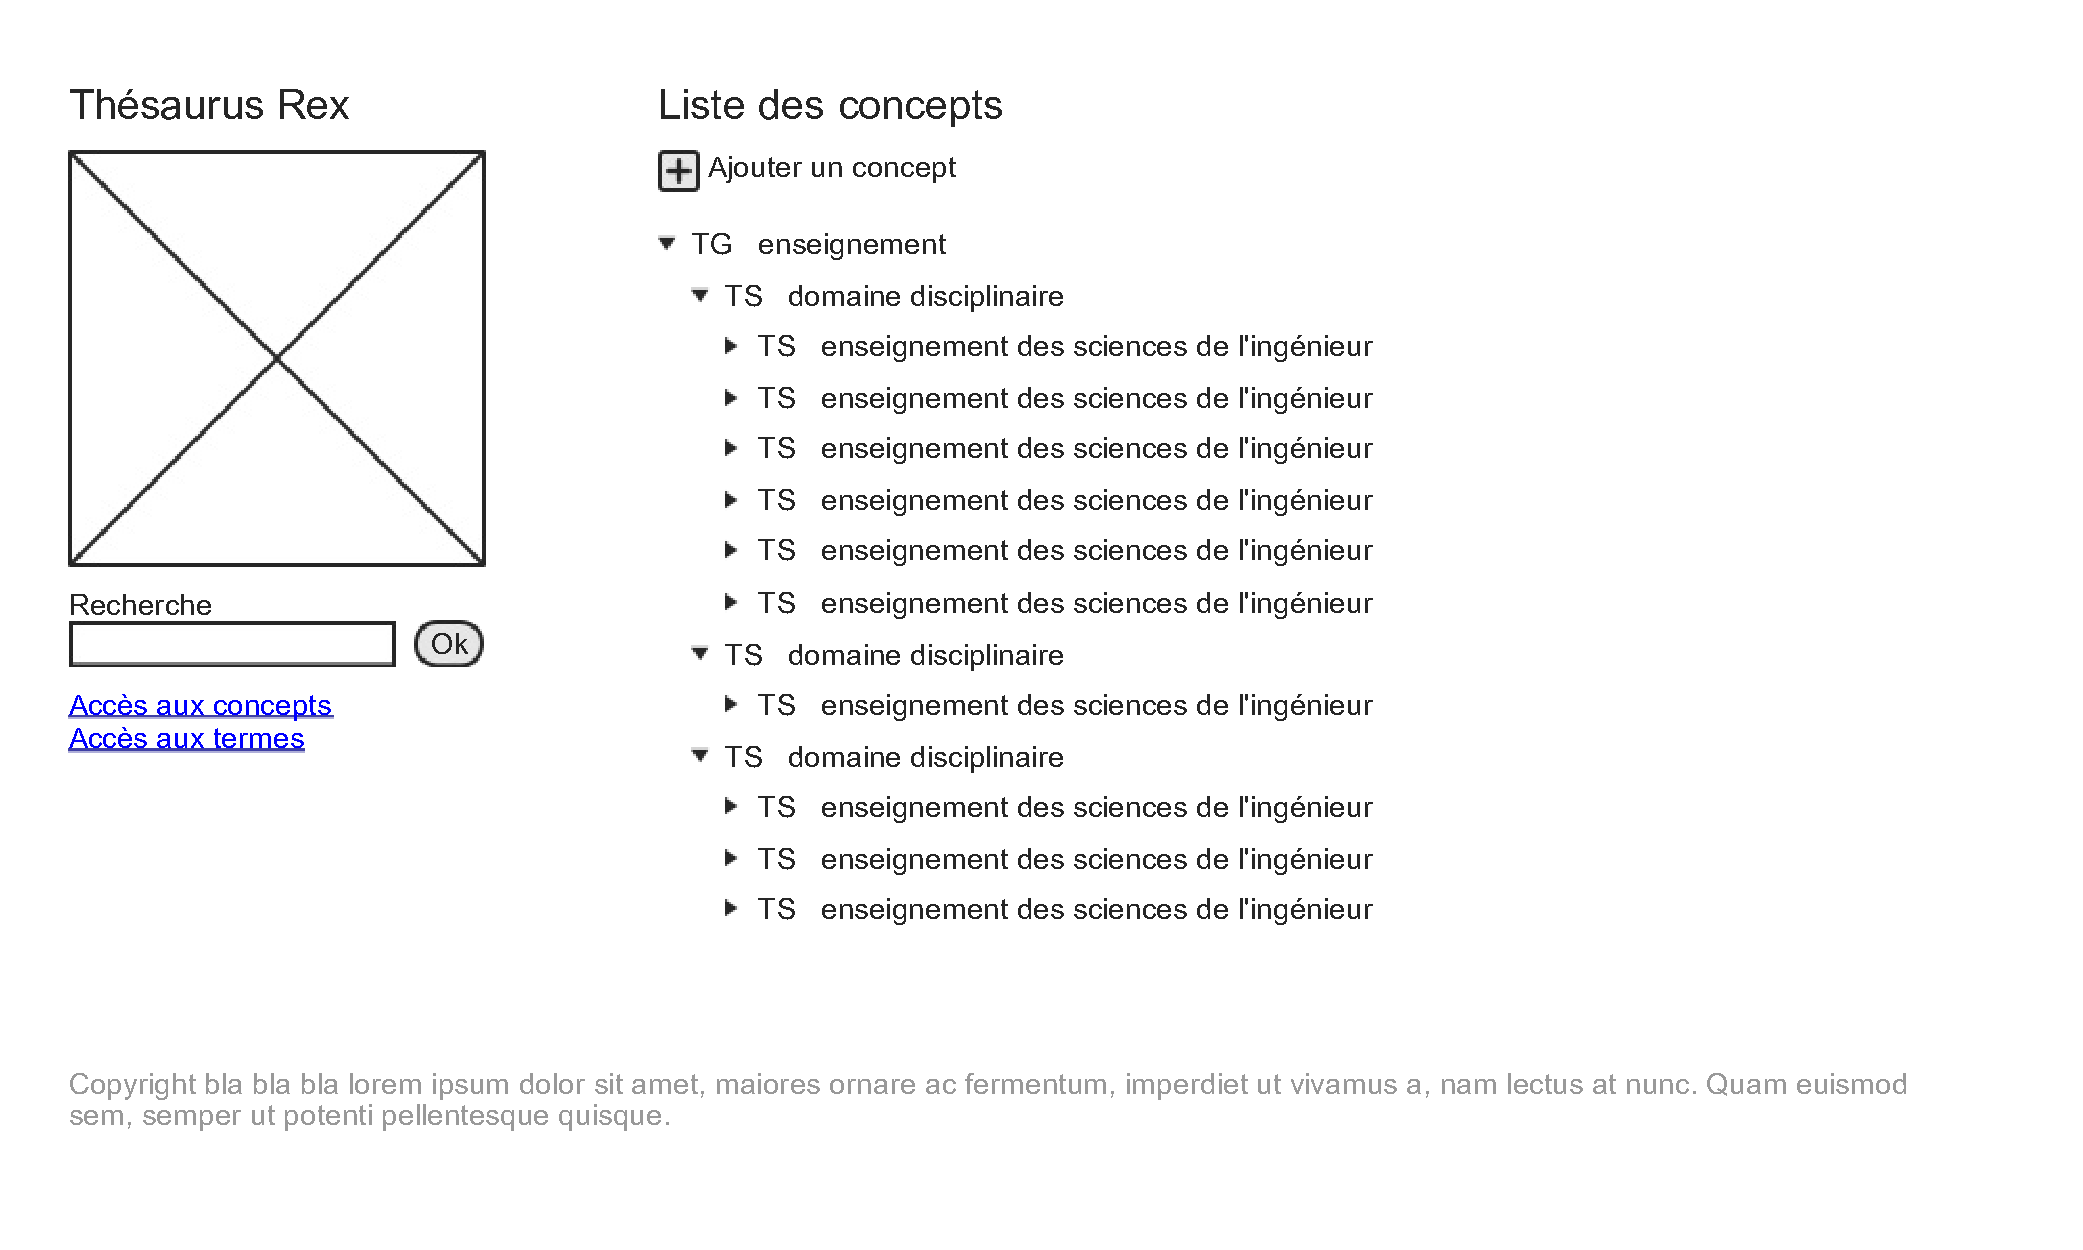
\includegraphics[width=\textwidth]{files/template_concepts}
\end{center}
\caption{Template de la vue hiérarchique des concepts.}
\end{figure}

\subsection{Visualisation d'un concept}

Lors du clique sur un concept à partir de la vue hiérarchique, le concept est affiché avec son environnement sémantique direct :
\begin{itemize}
\item son concept générique,
\item ses concepts spécifiques,
\item ses concepts associés,
\item ses termes synonymes.
\end{itemize}

Cette vue permet une navigation rapide dans la hiérarchie grâce à la multitude de liens.
\begin{figure}[H]
\begin{center}
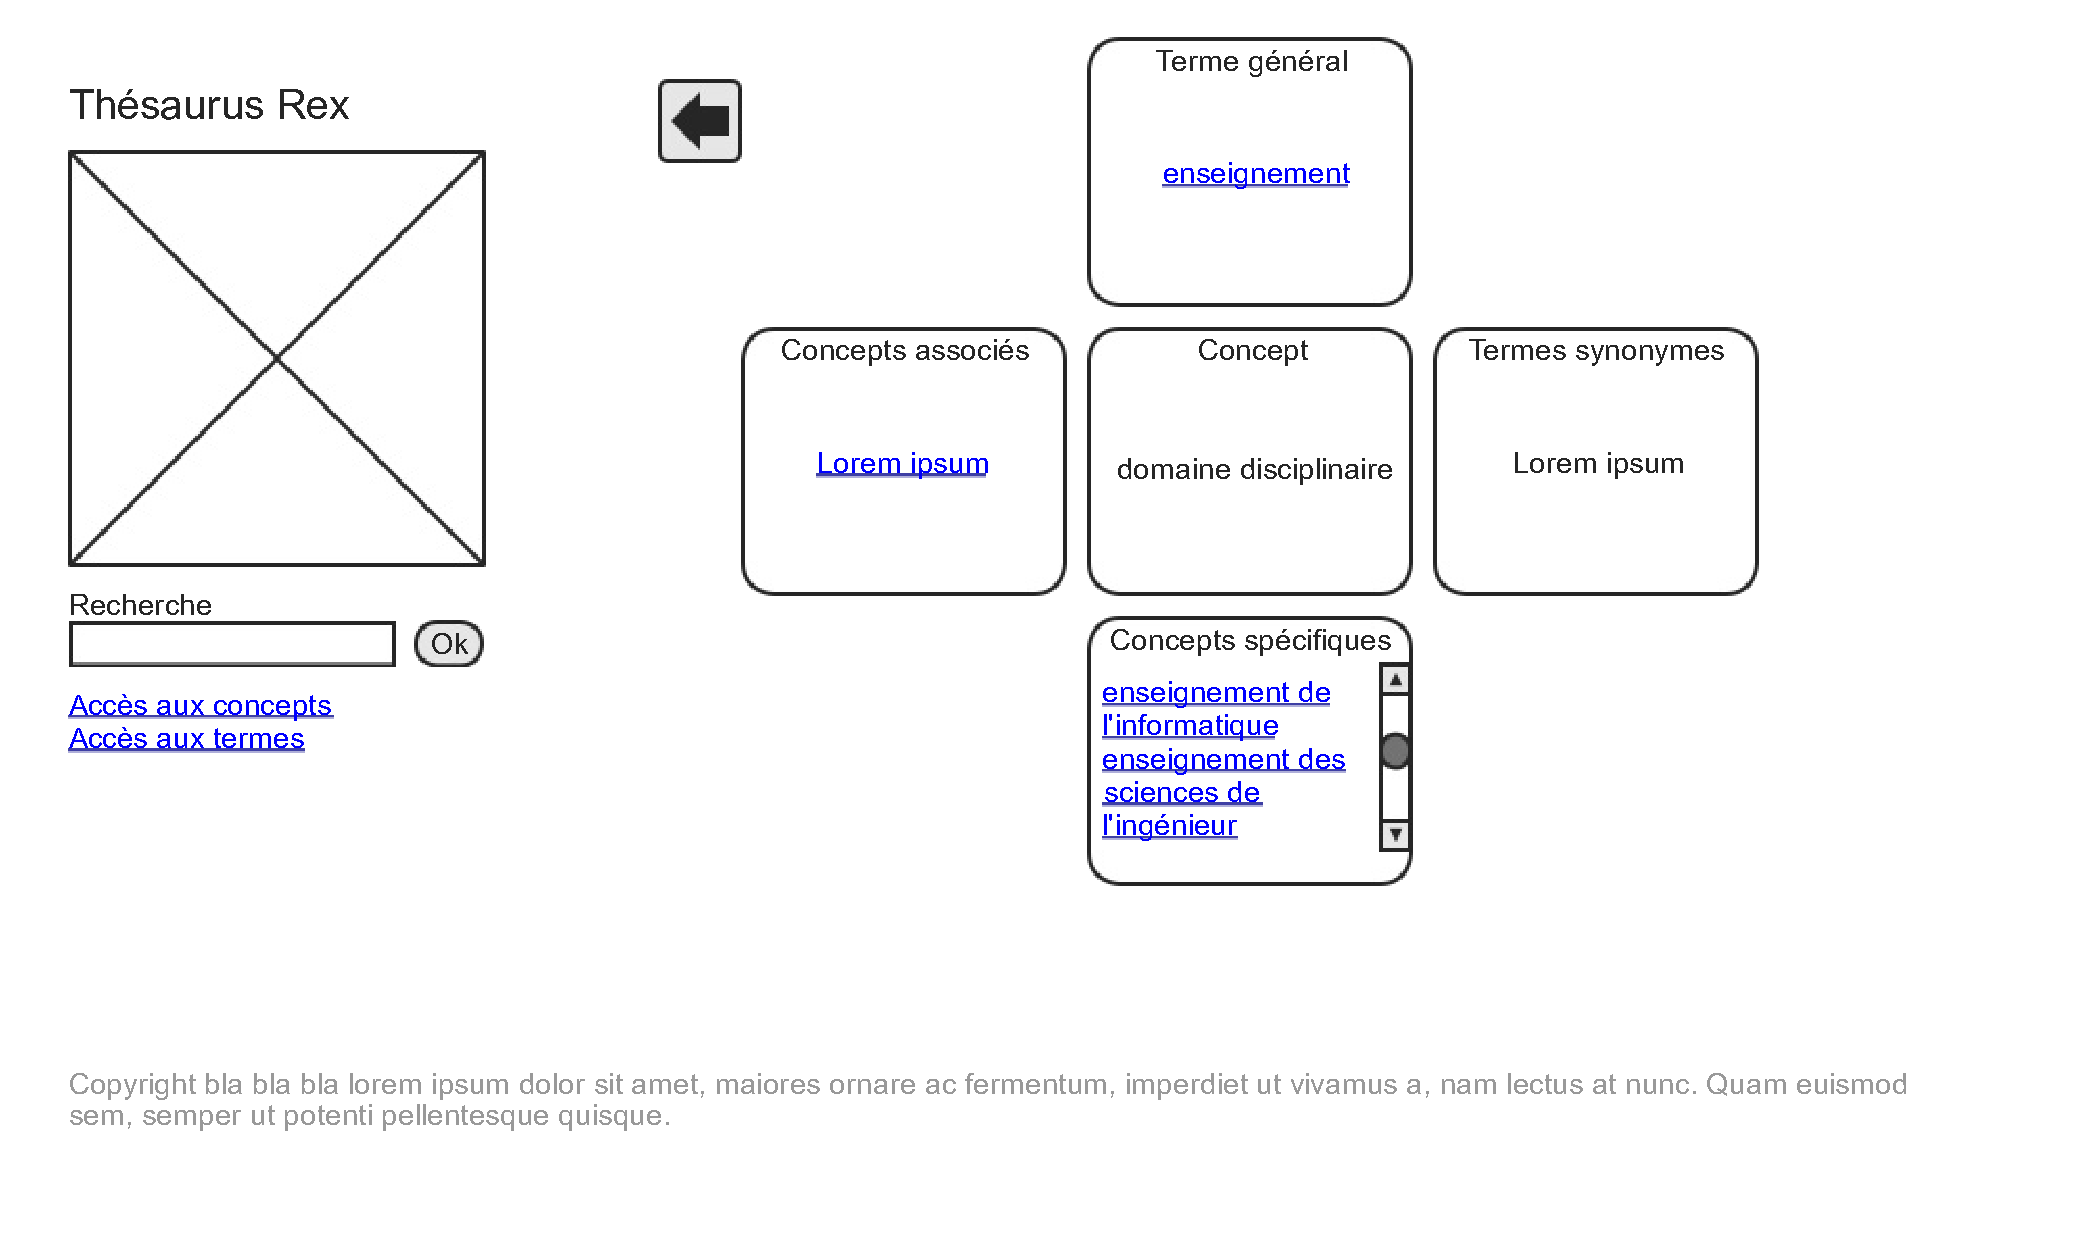
\includegraphics[width=\textwidth]{files/template_concept}
\end{center}
\caption{Template d'affichage d'un concept et de son environnement sémantique direct.}
\end{figure}

\subsection{Ajout / Édition d'un concept}

L'ajout et l'édition d'un concept se fait à l'aide des formulaires ci-après.
\begin{figure}[H]
\begin{center}
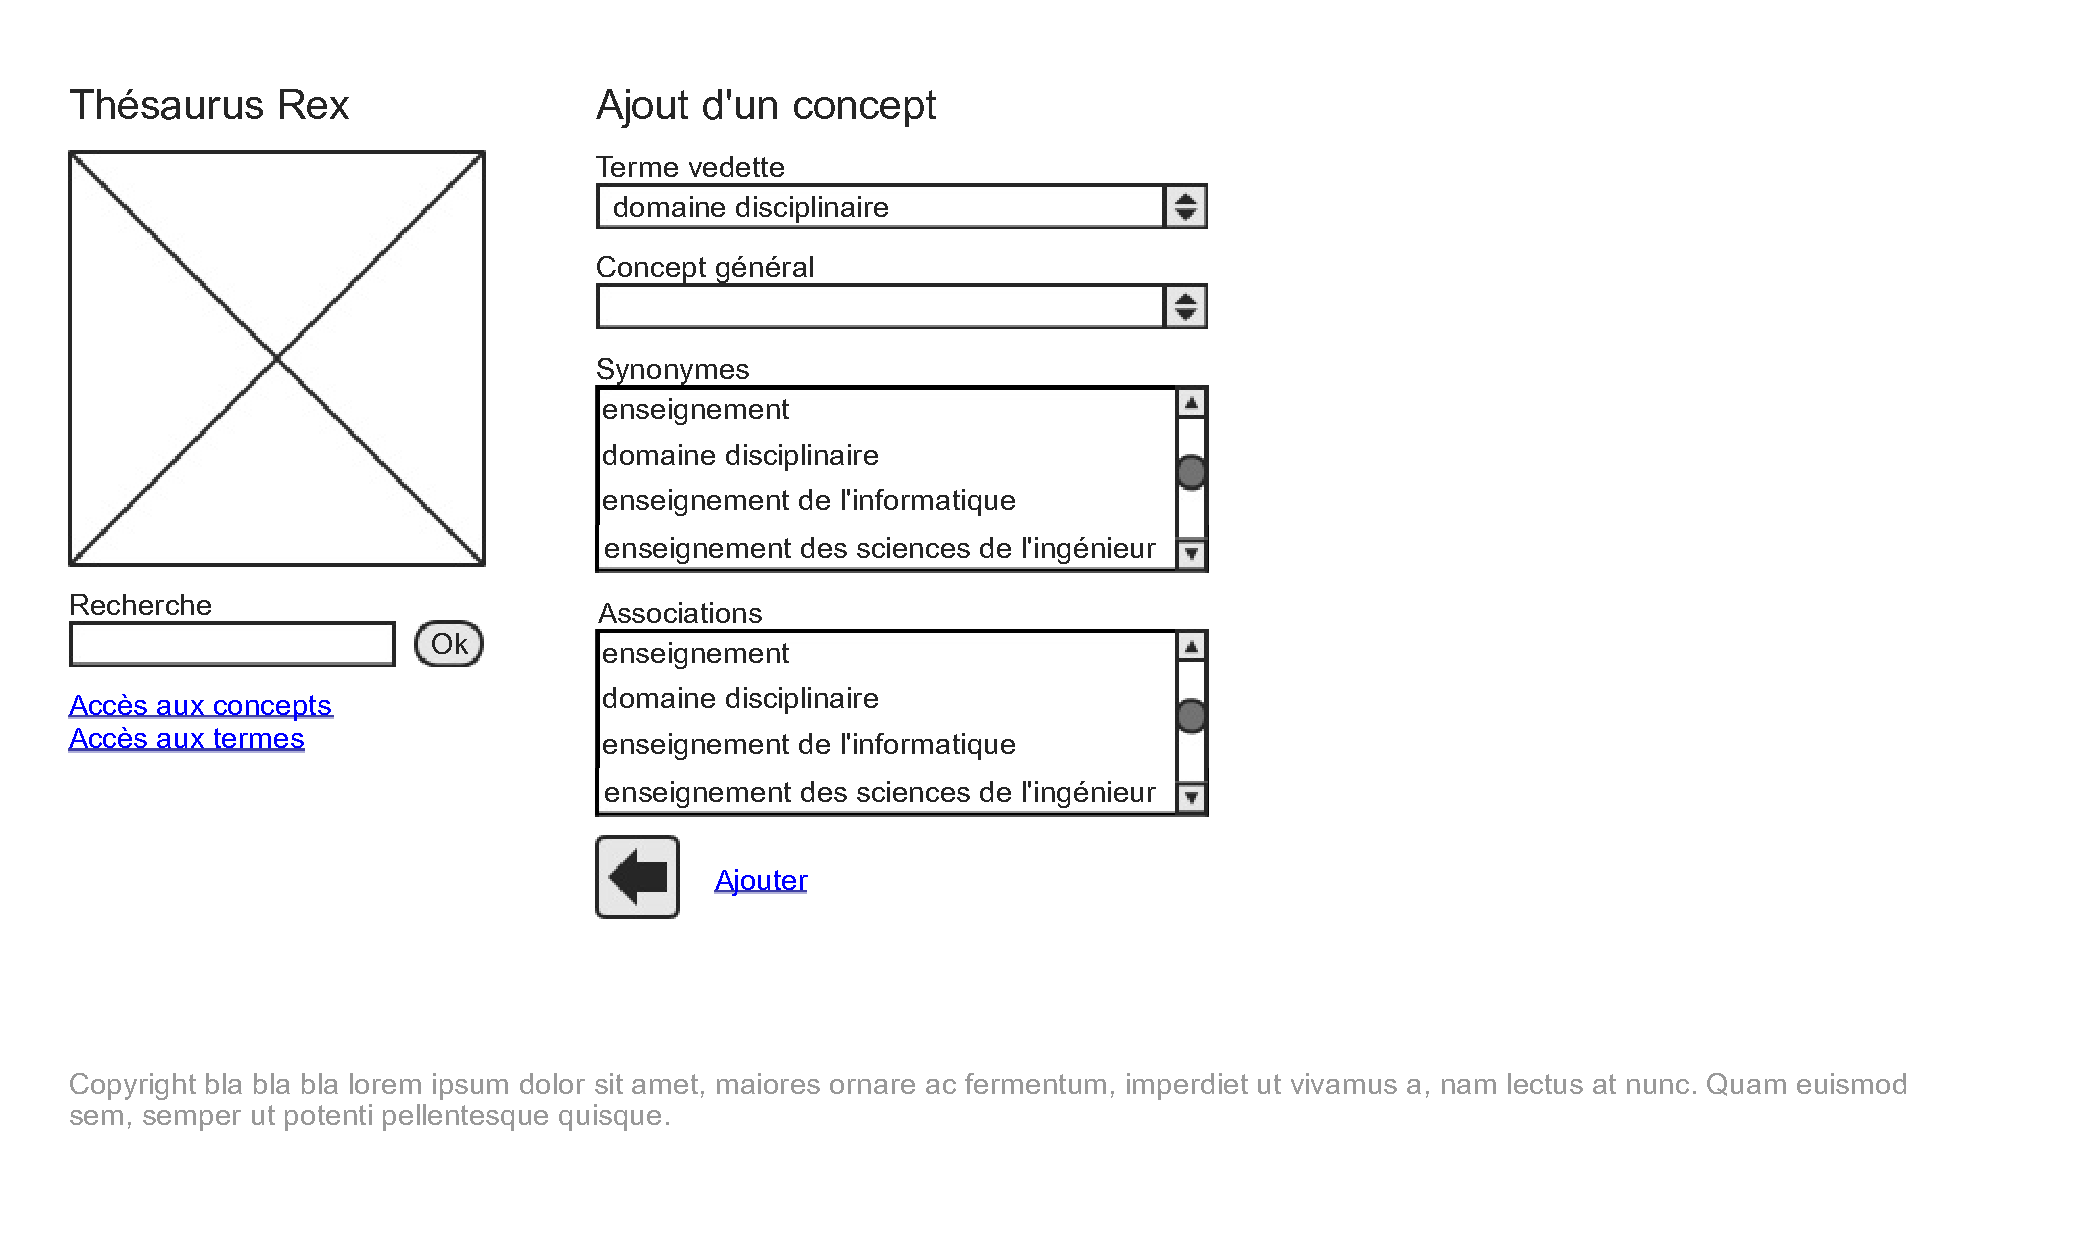
\includegraphics[width=\textwidth]{files/template_concept_add}
\end{center}
\caption{Template du formulaire d'ajout d'un concept.}
\end{figure}
\begin{figure}[H]
\begin{center}
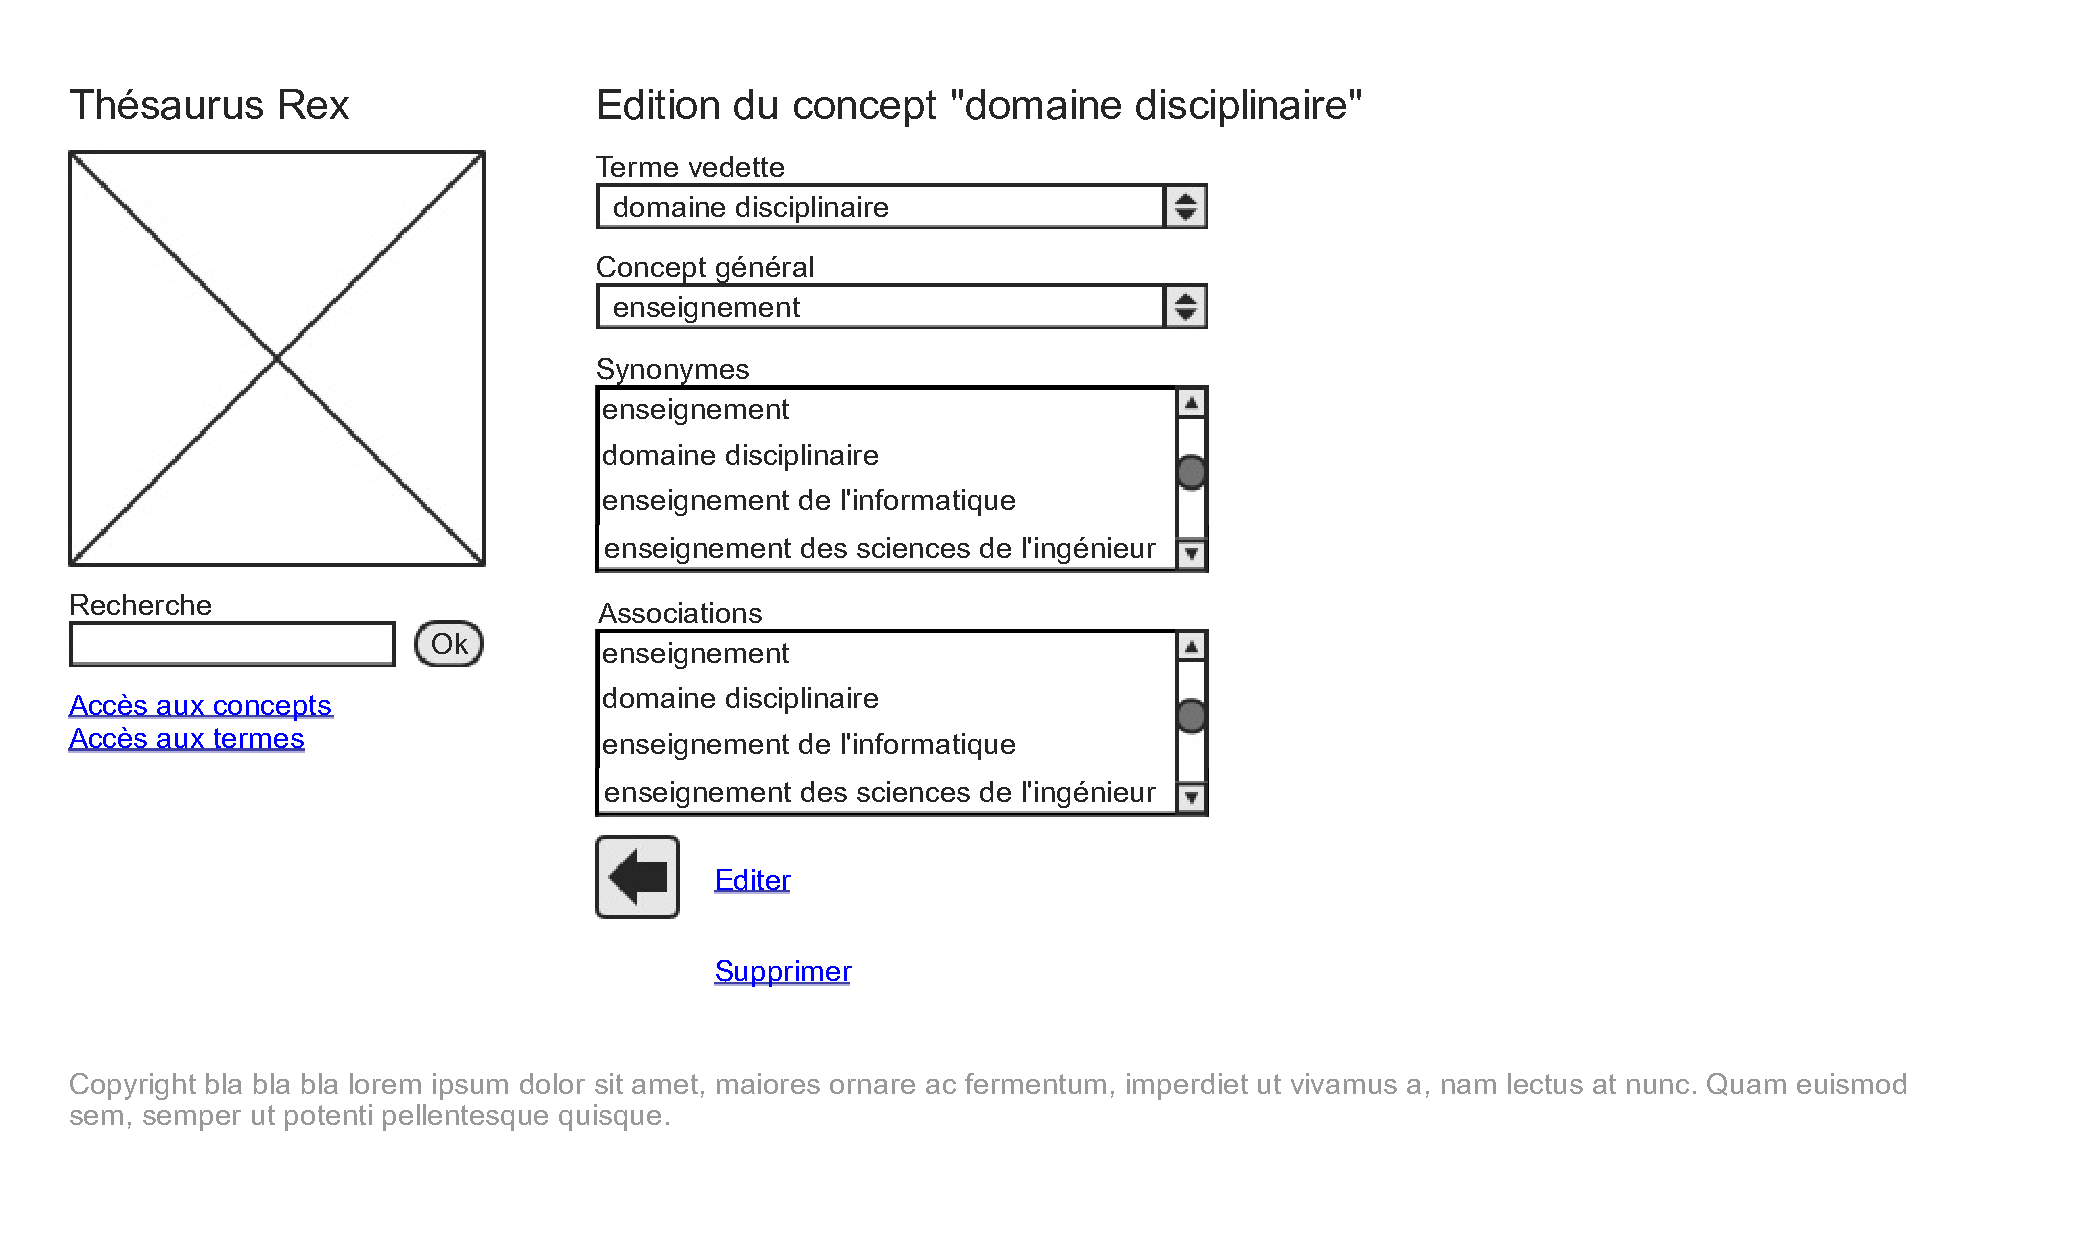
\includegraphics[width=\textwidth]{files/template_concept_edit}
\end{center}
\caption{Template du formulaire d’édition d'un concept.}
\end{figure}

\subsection{Liste des termes}

La seconde partie de l'application permet l'accès à la gestion des Termes. L'ensemble des termes peut être visualisé sous la forme d'une liste.
\begin{figure}[H]
\begin{center}
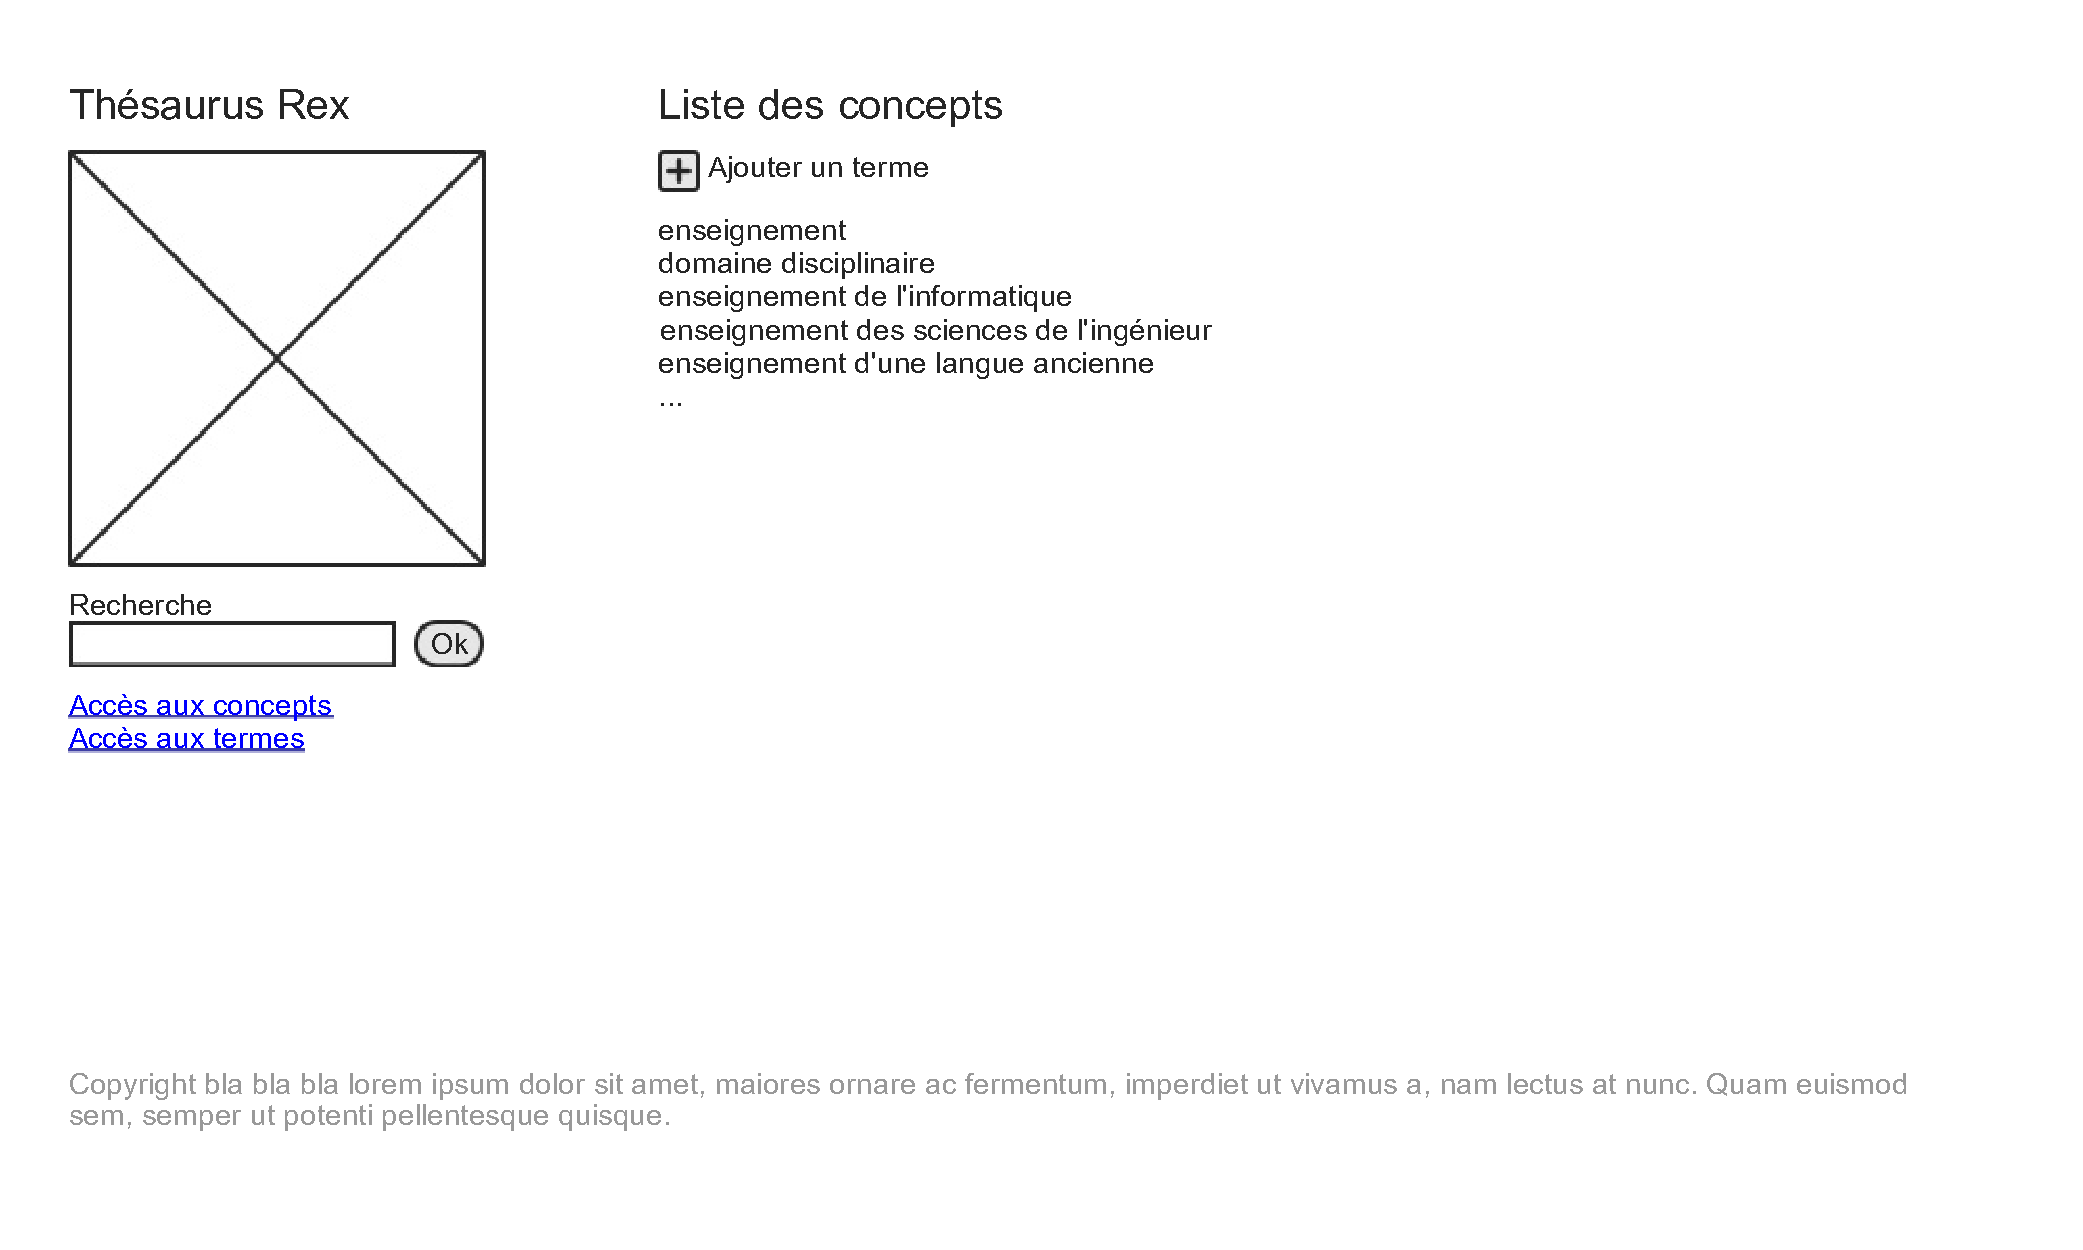
\includegraphics[width=\textwidth]{files/template_termes}
\end{center}
\caption{Template de visualisation des termes.}
\end{figure}

\subsection{Édition d'un terme}

Lors du clique sur un terme dans la liste, le formulaire d'édition suivant apparaît.
\begin{figure}[H]
\begin{center}
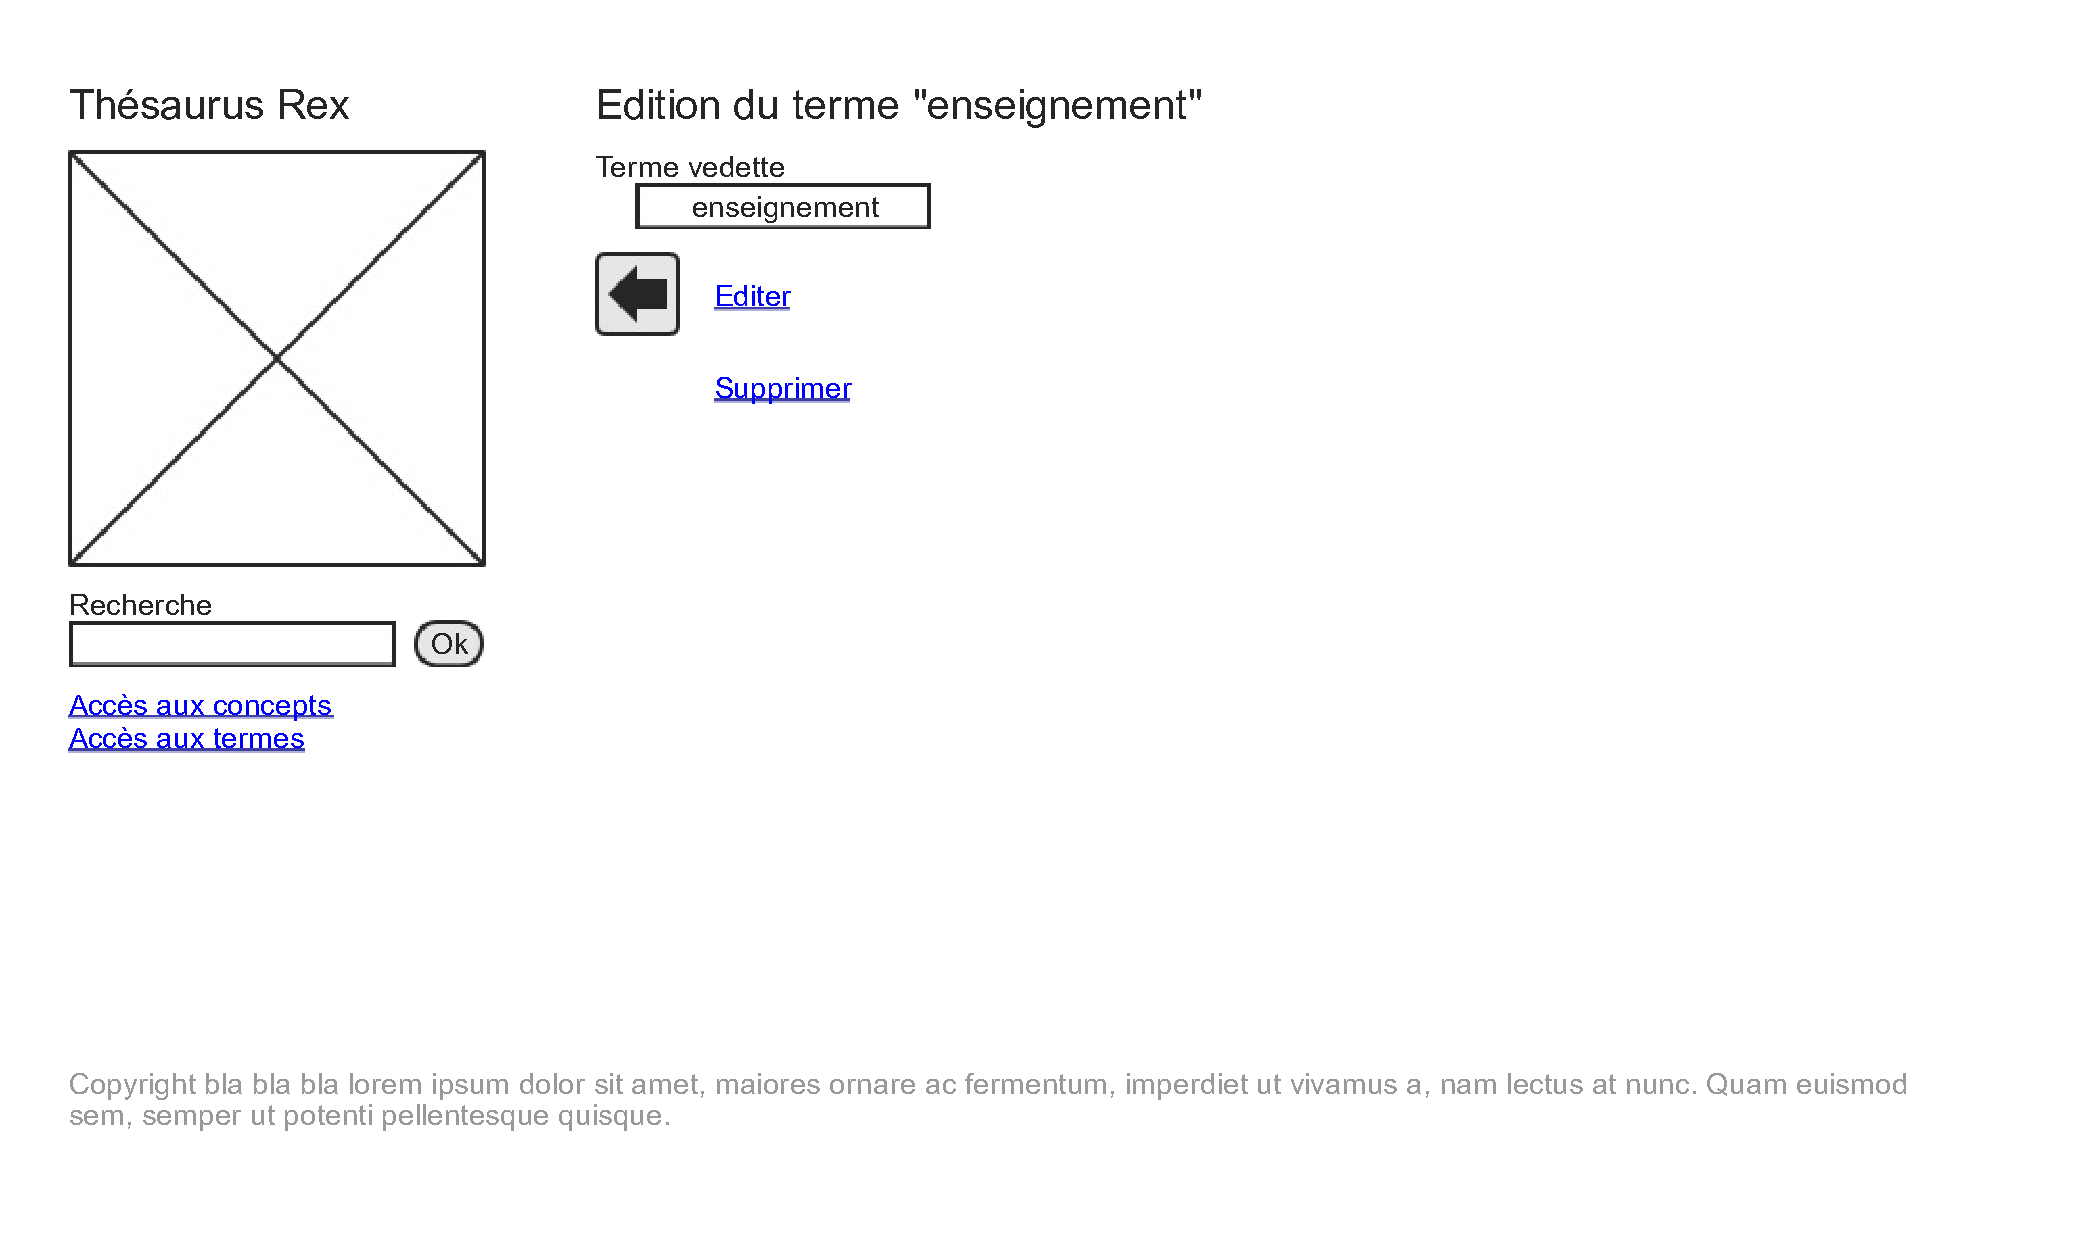
\includegraphics[width=\textwidth]{files/template_terme_edit}
\end{center}
\caption{Template du formulaire d'ajout d'un concept.}
\end{figure}
